\documentclass[conference]{IEEEtran}
\IEEEoverridecommandlockouts
\usepackage{cite}
\usepackage{amsmath,amssymb,amsfonts}
\usepackage{mathtools}
\usepackage{algorithmic}
\usepackage{graphicx}
\usepackage{booktabs}
\usepackage{textcomp}
\usepackage{xcolor}
\usepackage{url}
\usepackage{dblfloatfix}
\usepackage{placeins}
\allowdisplaybreaks[2]
\setcounter{topnumber}{3}
\setcounter{dbltopnumber}{2}
\renewcommand{\topfraction}{0.95}
\renewcommand{\dbltopfraction}{0.95}
\renewcommand{\textfraction}{0.05}
\renewcommand{\floatpagefraction}{0.80}
\renewcommand{\dblfloatpagefraction}{0.80}
\setlength{\textfloatsep}{10pt plus 2pt minus 2pt}
\setlength{\dbltextfloatsep}{10pt plus 2pt minus 2pt}
\DeclareMathOperator*{\argmin}{arg\,min}
\def\BibTeX{{\rm B\kern-.05em{\sc i\kern-.025em b}\kern-.08em
T\kern-.1667em\lower.7ex\hbox{E}\kern-.125emX}}

\title{RouteCast: Calibrated Cross-Token Expert Forecasting with Selective Cache-Aware Prefetching for Heterogeneous MoE Models}

\author{\IEEEauthorblockN{Jihua Dong}
\IEEEauthorblockA{\textit{School of Microelectronics} \\
\textit{University of Electronic Science and Technology of China}\\
Chengdu, China \\
2023190903038@std.uestc.edu.cn}}

\begin{document}
\maketitle

\begin{abstract}
Sparse mixture-of-experts (MoE) inference may transfer non-resident expert weights after routing, exposing data movement on the critical path. Prefetching can hide this movement only when forecasts arrive early and incorrect transfers do not overwhelm the cache. We present RouteCast, a route-only framework that forecasts next-token experts from previously observed selections without using hidden states or modifying the native router. A context-dependent gate combines popularity, transition, prefill, recurrent-history, and multiscale temporal evidence. Per-model temperature scaling then supports adaptive candidate budgets, confidence rejection, and cache-aware admission. Under request-disjoint limit=1000 evaluation, native-budget Recall reached 0.5558 on Qwen3, 0.3172 on DeepSeek-R1, and 0.3602 on Llama4 Maverick. These values exceed a matched temporal convolutional network baseline by 0.0281, 0.0455, and 0.0579, respectively. Confidence intervals from 10,000 paired request-level bootstrap resamples excluded zero for all three models. Trace-driven replay also reduced transfers relative to unfiltered adaptive-mass prefetching, although the cache-hit benefit depended on model and capacity. RouteCast therefore provides a calibrated interface between route forecasting and selective cache action. The trace-based evidence does not establish end-to-end latency gains in a deployed MoE system.
\end{abstract}

\begin{IEEEkeywords}
mixture of experts, expert prefetching, route prediction, calibration, adaptive budget, expert cache
\end{IEEEkeywords}

\section{Introduction}
Sparse MoE language models increase parameter capacity while evaluating only a small expert subset for each token. This conditional computation reduces arithmetic cost, but the complete expert pool can still exceed accelerator memory. In an offloaded deployment, an expert that is not resident must be transferred from host memory or another device after the native router selects it. Because the transfer lies between routing and expert execution, reactive loading can expose data-movement latency on the inference critical path.

Speculative expert prefetching attempts to move likely experts before they are demanded. Prior work has explored router co-design, proactive expert movement and sparsity-aware caching \cite{pregated,moeinfinity,promoe}. Public route traces further show that expert choices contain spatial and temporal structure \cite{patterns}. However, high prediction recall alone is insufficient: enlarging the candidate set trivially covers more true experts while increasing false transfers, cache pollution and replacement pressure. A useful predictor must therefore answer three linked questions: which experts are likely, how trustworthy is the score distribution, and which predictions should become physical prefetches under a finite cache budget?

We study these questions under a route-only constraint. RouteCast observes discrete expert identifiers from earlier token positions and structural metadata, but not hidden activations or native-router logits. This setting is attractive when traces are available across heterogeneous architectures or when modifying the serving model is undesirable. It is also difficult: Qwen3 and DeepSeek-R1 select eight experts from different pool sizes, whereas Llama4 Maverick selects one; consequently, a fixed heuristic or a predictor tuned to one routing regime need not transfer to the others.

RouteCast addresses this heterogeneity with six evidence branches and a context-dependent probability-mixture gate. The fused scores are calibrated separately for each model. A validation-selected probability-mass threshold controls the candidate budget, low-utility predictions can be rejected, and cache-aware admission prevents every high-ranked candidate from forcing a transfer. Figure~\ref{fig:framework} summarizes this progression from route observation to selective action.

RouteCast contributes a request-disjoint protocol for next-token expert forecasting across three heterogeneous public MoE trace families. Its shared predictor combines statistical transitions with learned temporal evidence without accessing hidden states. Per-model calibration, adaptive mass, and confidence rejection convert rankings into selective decisions. Trace-driven cache replay then measures downstream benefits and model--capacity failure boundaries. The evidence remains algorithmic; end-to-end latency, throughput, and energy are outside the present scope.

\begin{figure*}[!t]
\centering
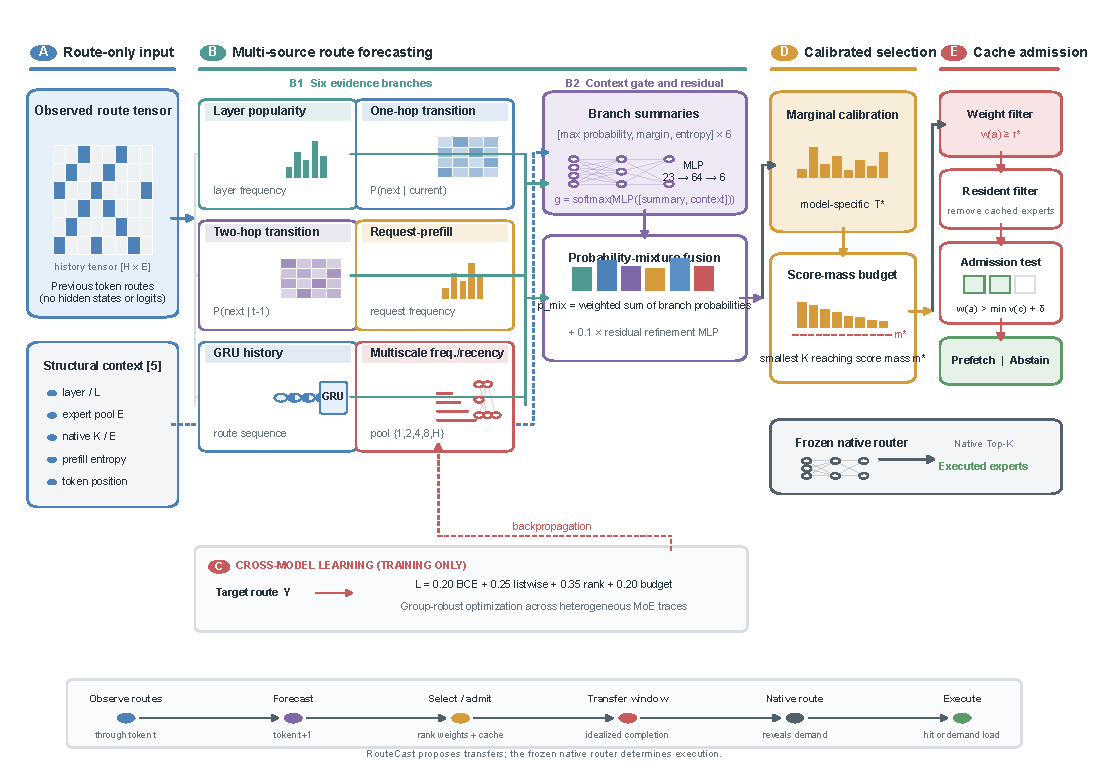
\includegraphics[width=0.98\textwidth]{figures/Fig1_routecast_framework}
\caption{RouteCast couples calibrated cross-token route forecasting to selective expert-prefetch decisions. Previously observed routes feed statistical and temporal predictors, a context gate combines their probability distributions, and calibration exposes a confidence-bearing interface for adaptive budget control and cache-aware admission. The native router remains authoritative.}
\label{fig:framework}
\end{figure*}
\FloatBarrier

\section{Related Work}
\textbf{MoE inference and expert movement.}
Pre-gated MoE jointly designs routing and execution to reduce inference overhead \cite{pregated}. MoE-Infinity exploits activation sparsity through expert caching on memory-constrained machines \cite{moeinfinity}, while ProMoE studies proactive caching for MoE serving \cite{promoe}. These systems motivate forecasting, but their reported system gains depend on deployment-specific overlap, bandwidth and cache behavior.

\textbf{Route forecasting.}
Patterns behind Chaos characterizes spatial and temporal regularities in expert-selection traces and provides the public data used in this study \cite{patterns}. Spatio-temporal prediction approaches similarly combine route relations across tokens or layers \cite{stmoe}. RouteCast differs in treating heterogeneous route statistics as conditionally useful evidence: a learned gate mixes normalized branch distributions rather than assigning one fixed fusion rule across models and requests.

\textbf{Prediction-aware prefetch decisions.}
Speculative prefetching studies increasingly emphasize that a prediction becomes useful only after accounting for its movement and residency consequences \cite{specmd,specprefetch}. RouteCast adopts this separation explicitly. Fixed-budget Recall and ranking metrics evaluate the forecaster; adaptive mass evaluates the candidate interface; and cache replay evaluates issued transfers. This prevents an increase in prediction coverage from being misreported as an equivalent systems speedup.

\section{RouteCast}
\subsection{Task Definition}
For request $r$, token position $t$ and routed layer $\ell$, let
$\mathcal{Y}_{r,t,\ell}\subseteq\{1,\ldots,E_r\}$ denote the native router's selected expert set, where $E_r$ is the model-specific expert count and $K_r=|\mathcal{Y}_{r,t,\ell}|$ is its native routing width. Given the route history up to token $t$, RouteCast predicts the next-token set at the corresponding routed layer:
\begin{equation}
\hat{\mathcal{Y}}_{r,t+1,\ell}
=f_\theta(\mathcal{R}_{r,1:t},\ell,\mathbf{c}_{r,t,\ell}).
\end{equation}
The predictor produces a score $s_{r,t,\ell,e}$ for every expert. For a candidate prefix $\mathcal{P}_{K}$,
\begin{equation}
\mathrm{Recall@K}=\frac{|\mathcal{P}_{K}\cap\mathcal{Y}|}{|\mathcal{Y}|},\quad
\mathrm{Precision@K}=\frac{|\mathcal{P}_{K}\cap\mathcal{Y}|}{K}.
\end{equation}
Native-budget evaluation uses $K=K_r$. Dynamic policies may issue fewer prefetches, including zero after confidence rejection.

\subsection{Six Route-Evidence Branches}
RouteCast constructs six per-expert signals:
\begin{equation}
\mathbf{z}_{t,\ell,e}=
[z^{\mathrm{pop}},z^{1\mathrm{hop}},z^{2\mathrm{hop}},
z^{\mathrm{pre}},z^{\mathrm{temp}},z^{\mathrm{multi}}]_{t,\ell,e}.
\end{equation}
Let $C_\ell(e)$ count training-set activations and $C_\ell^{(d)}(i,j)$ count transitions from expert $i$ to $j$ across a lag of $d$ tokens. The statistical branches are
\begin{align}
z^{\mathrm{pop}}_{t,\ell,e}
&=\frac{C_\ell(e)}{\sum_j C_\ell(j)},\\
z^{1\mathrm{hop}}_{t,\ell,e}
&=\frac{1}{|\mathcal{Y}_{t,\ell}|}
\sum_{i\in\mathcal{Y}_{t,\ell}}
\frac{C_\ell^{(1)}(i,e)}{\sum_jC_\ell^{(1)}(i,j)},\\
z^{2\mathrm{hop}}_{t,\ell,e}
&=\frac{1}{|\mathcal{Y}_{t-1,\ell}|}
\sum_{i\in\mathcal{Y}_{t-1,\ell}}
\frac{C_\ell^{(2)}(i,e)}{\sum_jC_\ell^{(2)}(i,j)}.
\label{eq:statistical-branches}
\end{align}
Zero-count rows fall back to layer popularity. If $C^{\mathrm{pre}}_{r,\ell}(e)$ counts activations in request $r$'s prefill, then
\begin{equation}
z^{\mathrm{pre}}_{t,\ell,e}=
\frac{C^{\mathrm{pre}}_{r,\ell}(e)}
{\sum_jC^{\mathrm{pre}}_{r,\ell}(j)},
\label{eq:prefill-branch}
\end{equation}
with the same fallback when the prefill count is empty.

For the learned branches, let $x_{u,\ell,e}=\mathbb{1}[e\in\mathcal{Y}_{u,\ell}]$. A shared per-expert GRU encodes the most recent $H=16$ indicators:
\begin{equation}
\mathbf{h}_{t,\ell,e}=\operatorname{GRU}
(x_{t-H+1:t,\ell,e}),\qquad
z^{\mathrm{temp}}_{t,\ell,e}=\mathbf{w}_h^\top\mathbf{h}_{t,\ell,e}+b_h.
\label{eq:temporal-branch}
\end{equation}
The multiscale feature vector contains window means and normalized recency,
\begin{align}
\mu_w(e)&=\frac{1}{w}\sum_{u=t-w+1}^{t}x_{u,\ell,e},
\quad w\in\{1,2,4,8,H\},\\
\mathbf{u}_{t,\ell,e}&=[\mu_1,\mu_2,\mu_4,\mu_8,\mu_H,d_{\mathrm{last}}],\\
z^{\mathrm{multi}}_{t,\ell,e}&=f_m(\mathbf{u}_{t,\ell,e}).
\label{eq:multiscale-branch}
\end{align}
The statistical branches provide stable priors; the learned branches capture request-specific temporal departures.

Each branch is normalized independently before fusion. For branch $b$,
\begin{equation}
p^{(b)}_{t,\ell,e}=
\frac{\exp(z^{(b)}_{t,\ell,e})}
{\sum_{j=1}^{E_r}\exp(z^{(b)}_{t,\ell,j})}.
\label{eq:branch-probability}
\end{equation}
This normalization makes branch outputs comparable even when their raw scales differ.

\subsection{Context-Dependent Probability Fusion}
Direct addition of branch logits is sensitive to incompatible score scales. RouteCast instead fuses the distributions in Eq.~\eqref{eq:branch-probability}. For each branch $b$, its confidence descriptor is
\begin{align}
H(p^{(b)})&=-\frac{1}{\log E_r}
\sum_e p^{(b)}_e\log(p^{(b)}_e+\epsilon),\\
\phi(p^{(b)})&=
\left[p^{(b)}_{(1)},\;p^{(b)}_{(1)}-p^{(b)}_{(2)},\;H(p^{(b)})\right].
\label{eq:branch-descriptor}
\end{align}
Concatenating the 18 branch statistics with structural context $\mathbf{c}_{t,\ell}$, comprising normalized layer position, expert-pool size, native sparsity, request entropy and token position, gives the gate input:
\begin{equation}
\mathbf{g}_{t,\ell}=\operatorname{softmax}
\!\left(f_g([\phi(\mathbf{z}_{t,\ell}),\mathbf{c}_{t,\ell}])\right).
\end{equation}
The fused expert score is
\begin{equation}
s_{t,\ell,e}=\log\!\left(\sum_b g^{(b)}_{t,\ell}
p^{(b)}_{t,\ell,e}+\epsilon\right)+\alpha r_{t,\ell,e},
\quad \alpha=0.1,
\label{eq:fusion}
\end{equation}
where $r_{t,\ell,e}=f_r(\mathbf{z}_{t,\ell,e},\mathbf{c}_{t,\ell})$ is a lightweight residual correction. This mixture can suppress evidence that is informative in one routing regime but harmful in another.

\subsection{Training Across Heterogeneous MoEs}
Let $y_e=\mathbb{1}[e\in\mathcal{Y}]$, $q_e=\sigma(s_e)$, $\pi_e=\operatorname{softmax}(s)_e$, and $\omega_+=(E_r-K_r)/K_r$. The predictor is trained with
\begin{equation}
\mathcal{L}=0.20\mathcal{L}_{\mathrm{BCE}}
+0.25\mathcal{L}_{\mathrm{list}}
+0.35\mathcal{L}_{\mathrm{rank}}
+0.20\mathcal{L}_{\mathrm{budget}}.
\label{eq:total-loss}
\end{equation}
The four terms are
\begin{align}
\mathcal{L}_{\mathrm{BCE}}
&=-\frac{1}{E_r}\sum_e\left[\omega_+y_e\log q_e+(1-y_e)\log(1-q_e)\right],\\
\mathcal{L}_{\mathrm{list}}
&=-\frac{1}{K_r\log E_r}\sum_e y_e\log\pi_e,\\
\mathcal{L}_{\mathrm{rank}}
&=\frac{1}{|\mathcal{Y}||\mathcal{N}_h|}
\sum_{i\in\mathcal{Y}}\sum_{j\in\mathcal{N}_h}
\operatorname{softplus}(s_j-s_i),\\
\mathcal{L}_{\mathrm{budget}}
&=\frac{1}{|\mathcal{K}|}\sum_{K\in\mathcal{K}}
\frac{1}{K_r}\sum_{i\in\mathcal{Y}}
\operatorname{softplus}(\kappa_K-s_i),
\label{eq:loss-components}
\end{align}
where $\mathcal{N}_h$ contains the 24 highest-scoring negative experts, $\mathcal{K}$ is the model-specific set of training budgets, and $\kappa_K$ is the $K$th-largest score. The budget surrogate penalizes true experts that fall below this cutoff.

Group distributionally robust optimization prevents the largest trace family from dominating training. Model-family weights are updated as
\begin{align}
w_g^{(u+1)}=
\frac{w_g^{(u)}\exp(\eta\mathcal{L}_g^{(u)})}
{\sum_h w_h^{(u)}\exp(\eta\mathcal{L}_h^{(u)})},\\
\mathcal{L}_{\mathrm{DRO}}=\sum_g w_g\mathcal{L}_g.
\label{eq:group-dro}
\end{align}
We use finite-value checks, FP32 loss reduction, float64 group-weight normalization, and gradient clipping. The stable limit=1000 run completed three epochs without non-finite parameters.

\subsection{Calibration and Adaptive Budget}
After freezing the predictor, each model receives a positive temperature selected by multilabel binary cross-entropy on validation requests. With $a_{t,\ell,e}(T)=\sigma(s_{t,\ell,e}/T)$,
\begin{align}
T_r^*=\argmin_{T>0}\sum_{(t,\ell)\in\mathcal{V}_r}\sum_e
\bigl[&-y_{t,\ell,e}\log a_{t,\ell,e}(T)\nonumber\\
&-(1-y_{t,\ell,e})\log(1-a_{t,\ell,e}(T))\bigr].
\label{eq:temperature-fit}
\end{align}
Reliability diagrams, BCE, Brier score, and ECE use $a(T_r^*)$. Cumulative-mass selection additionally requires a categorical distribution over experts, so the same frozen temperature defines
\begin{equation}
\tilde p_{t,\ell,e}=
\frac{\exp(s_{t,\ell,e}/T_r^*)}
{\sum_j\exp(s_{t,\ell,j}/T_r^*)}.
\label{eq:mass-probability}
\end{equation}
Temperature scaling leaves expert ranking unchanged but changes the probability concentration used by downstream decisions. For cumulative mass $m$, RouteCast selects
\begin{equation}
K_{t,\ell}(m)=\min\left\{k:\sum_{i=1}^{k}
\tilde p_{t,\ell,(i)}\ge m\right\}.
\end{equation}
In budget-preserving mode, $K_{t,\ell}$ is capped by the model's native routing width. Validation selects the smallest average budget that retains a prescribed fraction $\rho$ of fixed-native validation recall:
\begin{equation}
m^*=\argmin_m\overline{K}(m)\quad
\mathrm{s.t.}\quad R_{\mathrm{val}}(m)\ge
\rho R_{\mathrm{val}}(K_r),\quad \rho=0.98.
\label{eq:mass-selection}
\end{equation}

\subsection{Confidence Rejection and Cache-Aware Admission}
Ranking candidates does not require issuing every candidate. A validation-selected threshold $\tau$ retains
\begin{equation}
\mathcal{A}_{t,\ell}=\{e\in\operatorname{TopK}
(\tilde p,K_{t,\ell}):\tilde p_{t,\ell,e}\ge\tau\},
\end{equation}
where $\tau$ maximizes useful prefetches minus a weighted count of wasted prefetches. A threshold above one is allowed, enabling complete abstention when all evaluated prefetches have negative validation utility.

More precisely, validation chooses
\begin{equation}
\tau_r^*=\argmax_{\tau\in\mathcal{Q}}
\frac{N_{\mathrm{use}}(\tau)-lambda_wN_{\mathrm{waste}}(\tau)}
{N_{\mathrm{val}}},
\label{eq:abstention-utility}
\end{equation}
with $\lambda_w=1$ in the reported replay. Ties prefer fewer issued prefetches and then the larger threshold.

Let $\mathcal{C}_{t}$ be the resident cache. RouteCast first removes resident candidates, $\mathcal{N}_{t,\ell}=\mathcal{A}_{t,\ell}\setminus\mathcal{C}_{t}$. A resident entry $c$ is refreshed by
\begin{equation}
v_t(c)=
\begin{cases}
\tilde p_{t,\ell,e}, & c=(\ell,e)\text{ is scored at }t,\\
\beta v_{t-1}(c), & \text{otherwise},
\end{cases}
\qquad \beta=0.90.
\label{eq:cache-value}
\end{equation}
If capacity is available, a non-resident candidate is admitted directly. Otherwise, candidate $a$ replaces the minimum-value resident entry $c^*$ only if
\begin{equation}
c^*=\argmin_{c\in\mathcal{C}_t}v_t(c),
\qquad \tilde p_t(a)>v_t(c^*)+\delta,
\label{eq:cache-admission}
\end{equation}
where $\delta=0$ in the reported experiments. This rule separates forecasting from physical action. The native router remains authoritative, and a mistaken forecast affects only speculative movement.

\section{Experimental Methodology}
\subsection{Trace Data and Split Protocol}
We use public expert-selection traces associated with Patterns behind Chaos \cite{patterns}. The evaluated families are Qwen3-235B-A22B, DeepSeek-R1 and Llama4 Maverick. They expose 128, 256 and 128 experts, respectively; Qwen3 and DeepSeek-R1 use native Top-8 routing, whereas Llama4 uses Top-1. For each family, at most 1,000 complete requests are assigned to train, validation or test by a deterministic hash of the relative request identifier. All token-layer records from a request remain in one split. The resulting packed cache contains 22,376,230 examples across 3,000 request files; its full numeric audit found no non-finite tensors.

\subsection{Baselines and Metrics}
The main forecasting baselines are Paper Heatmap, a request-aware heatmap, a history-only GRU, and a history-only temporal convolutional network (TCN). All learned methods use the same split, targets, multi-budget loss, and Group-DRO protocol. Paper Heatmap estimates cross-token transition statistics following the trace paper, whereas the request-aware version additionally conditions statistics on the current request. GRU-only uses recurrent history, and TCN-only applies four causal dilated-convolution blocks with dilation factors 1, 2, 4, and 8. Neither neural baseline receives RouteCast's statistical, prefill, or context-gated fusion features. We report Recall@K, Precision@K, mean true experts in the predicted set, mean reciprocal rank (MRR) and normalized discounted cumulative gain (NDCG). Because native-budget prediction and the true set have equal cardinality, Recall and Precision are numerically equal in Table~\ref{tab:main}.

For ranked list $\pi$ and binary relevance $y$, the ranking metrics are
\begin{align}
\mathrm{MRR}&=\frac{1}{N}\sum_{n=1}^{N}
\frac{1}{\min\{i:y_{n,\pi_i}=1\}},\\
\mathrm{DCG}_{n,K}&=\sum_{i=1}^{K}
\frac{y_{n,\pi_i}}{\log_2(i+1)},\\
\mathrm{IDCG}_{K}&=\sum_{i=1}^{\min(K,K_r)}
\frac{1}{\log_2(i+1)},\\
\mathrm{NDCG@K}&=\frac{1}{N}\sum_{n=1}^{N}
\frac{\mathrm{DCG}_{n,K}}{\mathrm{IDCG}_{K}}.
\label{eq:ranking-metrics}
\end{align}

Uncertainty is assessed by paired bootstrap over requests rather than token-layer examples. Each of 10,000 resamples draws complete test requests with replacement and recomputes the pooled metric. This preserves within-request dependence and uses seed 2026.

\subsection{Development and Replay Experiments}
The stable limit=1000 experiment supplies the main forecasting result. Limit=100 experiments are used for module ablation, budget curves, calibration development, three-seed screening and cache replay. Cache replay evaluates LRU, fixed native-budget prefetching, unfiltered adaptive-mass prefetching and the full adaptive cache-aware policy at cache capacities of $1\times$, $2\times$ and $4\times$ the native working-set reference. We report hit rate, total expert transfers and prefetch precision. Replay does not simulate kernel execution or overlap and therefore cannot establish latency or throughput gains.

Let $N_{\mathrm{hit}}$ and $N_{\mathrm{miss}}$ count demand accesses, $N_{\mathrm{pf}}$ count speculative loads, and $N_{\mathrm{use}}$ count prefetched experts subsequently demanded before eviction. Replay reports
\begin{align}
H_{\mathrm{cache}}&=
\frac{N_{\mathrm{hit}}}{N_{\mathrm{hit}}+N_{\mathrm{miss}}},\\
N_{\mathrm{transfer}}&=N_{\mathrm{miss}}+N_{\mathrm{pf}},\\
P_{\mathrm{pf}}&=
\frac{N_{\mathrm{use}}}{\max(1,N_{\mathrm{pf}})}.
\label{eq:cache-metrics}
\end{align}

\begin{figure*}[!t]
\centering
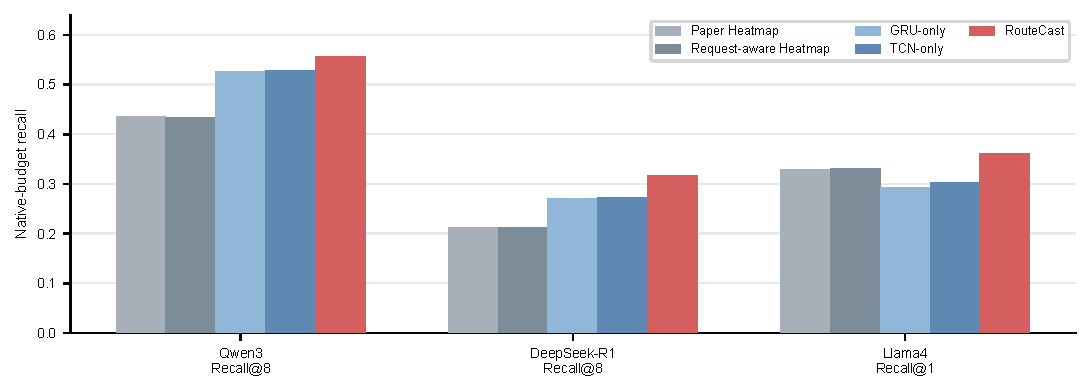
\includegraphics[width=0.92\textwidth]{figures/split/Fig2a_main_grouped_comparison}
\caption{Native-budget Recall under the stable limit=1000 protocol. Grouped bars preserve the same method encoding across Qwen3, DeepSeek-R1 and Llama4 Maverick without shrinking three independent axes into one composite.}
\label{fig:main}
\end{figure*}

\section{Results}
\subsection{RouteCast Improves Native-Budget Forecasting}
Table~\ref{tab:main} and Fig.~\ref{fig:main} report the stable limit=1000 result. RouteCast achieved Recall@8 of 0.5558 on Qwen3 and 0.3172 on DeepSeek-R1, and Recall@1 of 0.3602 on Llama4 Maverick. It was the best evaluated method for every model and metric. TCN-only slightly exceeded GRU-only on native-budget Recall, making it the stronger temporal baseline. RouteCast exceeded TCN-only by 0.0281, 0.0455, and 0.0579 on the three models. The corresponding paired request-level 95\% bootstrap intervals were $[0.0265,0.0299]$, $[0.0403,0.0510]$, and $[0.0546,0.0610]$; all excluded zero. RouteCast also exceeded GRU-only by 0.0290, 0.0467, and 0.0665. These comparisons show that the gain cannot be attributed solely to recurrent or convolutional encoding of route history.

We additionally repeated matched RouteCast and TCN training with seeds 2024, 2025, and 2026 in the limit=100 development setting. RouteCast exceeded TCN for every model under every seed. Its mean Recall advantage was $0.0317\pm0.0017$ on Qwen3, $0.0196\pm0.0062$ on DeepSeek-R1, and $0.0219\pm0.0041$ on Llama4 Maverick (mean $\pm$ sample standard deviation across seeds; Fig.~\ref{fig:tcn-seeds}). This screening supports optimization stability, while the request-level bootstrap on limit=1000 remains the primary uncertainty analysis.

\begin{table}[!t]
\centering
\caption{Native-budget limit=1000 results. Precision equals Recall at native K.}
\label{tab:main}
\scriptsize
\setlength{\tabcolsep}{2.4pt}
\begin{tabular}{llccc}
\toprule
Model & Method & Recall & MRR & NDCG \\
\midrule
Qwen3 & Heatmap & .4352 & .7969 & .4859 \\
& Request-aware & .4330 & .7956 & .4834 \\
& GRU-only & .5268 & .8893 & .5903 \\
& TCN-only & .5277 & .8902 & .5936 \\
& \textbf{RouteCast} & \textbf{.5558} & \textbf{.9013} & \textbf{.6208} \\
\midrule
DeepSeek-R1 & Heatmap & .2131 & .5087 & .2413 \\
& Request-aware & .2121 & .5076 & .2402 \\
& GRU-only & .2705 & .6715 & .3243 \\
& TCN-only & .2717 & .6707 & .3265 \\
& \textbf{RouteCast} & \textbf{.3172} & \textbf{.7131} & \textbf{.3743} \\
\midrule
Llama4 & Heatmap & .3298 & .4593 & .3298 \\
& Request-aware & .3311 & .4653 & .3311 \\
& GRU-only & .2938 & .4470 & .2938 \\
& TCN-only & .3024 & .4451 & .3024 \\
& \textbf{RouteCast} & \textbf{.3602} & \textbf{.4988} & \textbf{.3602} \\
\bottomrule
\end{tabular}
\end{table}

\begin{figure}[!t]
\centering
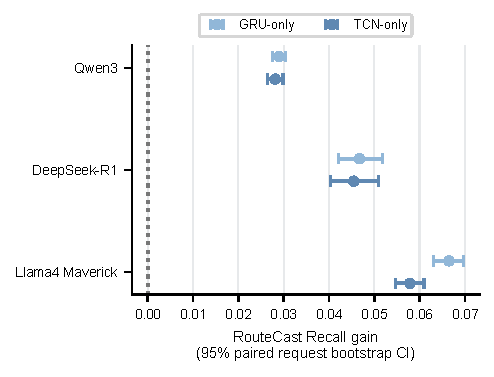
\includegraphics[width=0.92\columnwidth]{figures/split/Fig2b_paired_bootstrap}
\caption{Absolute RouteCast Recall gains over GRU-only and TCN-only with 95\% paired request-level bootstrap confidence intervals. Each resample draws complete test requests with replacement.}
\label{fig:bootstrap}
\end{figure}
\FloatBarrier

\begin{figure}[!t]
\centering
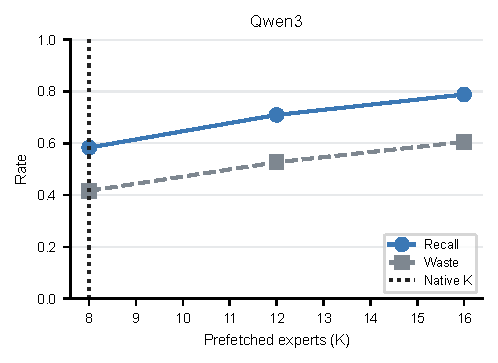
\includegraphics[width=0.94\columnwidth]{figures/split/Fig3_budget_qwen3}
\caption{Qwen3 budget--quality trade-off.}
\label{fig:budget_qwen}
\end{figure}
\begin{figure}[!t]
\centering
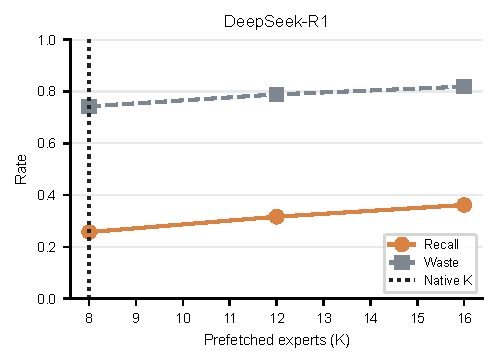
\includegraphics[width=0.94\columnwidth]{figures/split/Fig3_budget_deepseek_r1}
\caption{DeepSeek-R1 budget--quality trade-off.}
\label{fig:budget_deepseek}
\end{figure}
\begin{figure}[!t]
\centering
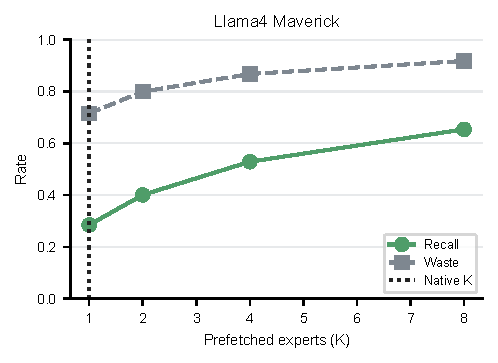
\includegraphics[width=0.94\columnwidth]{figures/split/Fig3_budget_llama4_maverick}
\caption{Llama4 Maverick budget--quality trade-off. Vertical dotted lines in Figs.~\ref{fig:budget_qwen}--\ref{fig:budget_llama} mark native K.}
\label{fig:budget_llama}
\end{figure}

\subsection{Budget Expansion Reveals Model-Specific Cost}
Increasing the number of prefetched experts raised coverage for every model, but the gain came with rapidly increasing waste (Figs.~\ref{fig:budget_qwen}--\ref{fig:budget_llama}). For Qwen3, moving from $K=8$ to 16 increased Recall from 0.5835 to 0.7886 while waste rose from 0.4165 to 0.6057. DeepSeek-R1 remained substantially harder: Recall rose from 0.2572 to only 0.3618 and waste reached 0.8191 at $K=16$. For Llama4, increasing $K$ from 1 to 8 raised Recall from 0.2848 to 0.6540, but 91.8\% of prefetched experts were false positives. These curves rule out ``prefetch more'' as a sufficient solution and motivate calibrated selection and abstention.
\FloatBarrier

\begin{figure}[!t]
\centering
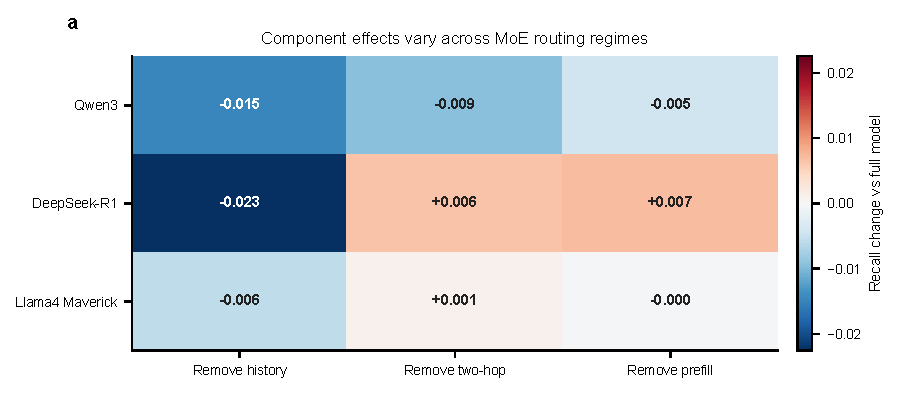
\includegraphics[width=0.96\columnwidth]{figures/Fig4_cross_model_ablation}
\caption{Native-budget Recall change after removing individual RouteCast components. Results use the limit=100 development split.}
\label{fig:ablation}
\end{figure}

\subsection{Component Utility Depends on the Routing Regime}
Cross-token history was the only ablated component whose removal degraded all three models (Fig.~\ref{fig:ablation}). Removing it reduced Recall by 0.0148 on Qwen3, 0.0226 on DeepSeek-R1 and 0.0056 on Llama4. Two-hop and prefill features helped Qwen3 but were neutral or harmful for the other families. In particular, removing two-hop or prefill evidence improved DeepSeek-R1 by approximately 0.0064 and 0.0069. The result supports conditional fusion rather than the stronger claim that every branch is universally beneficial.
\FloatBarrier

\subsection{Calibration Enables Adaptive Candidate Selection}
Temperature scaling served two distinct purposes. First, it measured whether the score magnitude represented expert-membership confidence. Second, it controlled how quickly the categorical probability accumulated and therefore how many candidates satisfied Eq.~\eqref{eq:mass-selection}. Since temperature does not alter score order, any change in dynamic width comes from probability concentration rather than improved ranking.

The fitted temperatures differed sharply across models: 0.82 for Qwen3, 0.32 for DeepSeek-R1, and 1.05 for Llama4 Maverick. Figure~\ref{fig:calibration-budget}a shows the corresponding test ECE. Scaling reduced ECE from 0.2894 to 0.2801 on Qwen3 and from 0.3827 to 0.2763 on DeepSeek-R1. For Llama4 Maverick, ECE changed from 0.1236 to 0.1250, a slight deterioration. Thus, temperature scaling substantially corrected DeepSeek-R1 confidence but did not improve every model. The low DeepSeek-R1 temperature indicates that its logits required sharpening; it does not imply higher forecasting accuracy.

Validation then selected masses of 0.70, 0.95, and 0.50 for Qwen3, DeepSeek-R1, and Llama4 Maverick, respectively (Fig.~\ref{fig:calibration-budget}b). These choices produced average candidate widths of 11.75, 17.25, and 6.56, with validation Recall of 0.6120, 0.3786, and 0.6293. DeepSeek-R1 therefore required both the highest cumulative mass and the widest candidate set, yet achieved the lowest Recall. This result identifies a routing-regime limitation rather than a calibration failure: reshaping confidence cannot recover information absent from the route history. The model-specific operating points also rule out one global mass threshold as a reliable cross-architecture policy.

\begin{figure*}[!t]
\centering
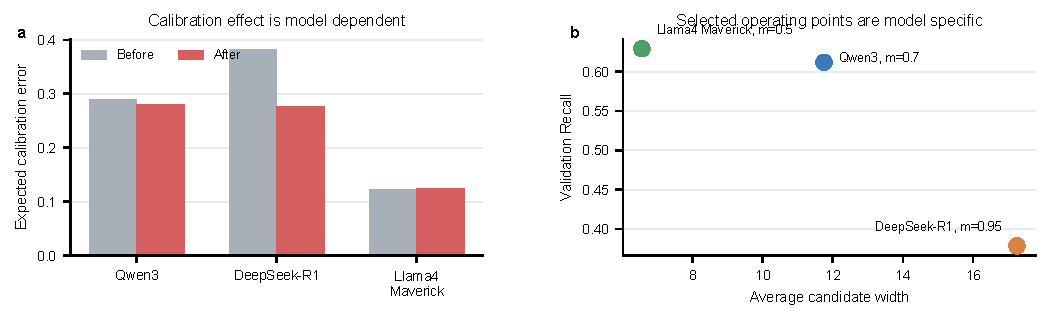
\includegraphics[width=0.92\textwidth]{figures/compact/Fig5_compact_calibration_budget}
\caption{Calibration and adaptive-budget selection. (a) Test expected calibration error before and after per-model temperature scaling. Lower is better. Scaling strongly improves DeepSeek-R1, modestly improves Qwen3, and slightly worsens Llama4 Maverick. (b) Validation-selected operating points. Labels report cumulative mass; coordinates show the resulting average candidate width and Recall. Full reliability diagrams and mass sweeps are provided in the supplementary figure package.}
\label{fig:calibration-budget}
\end{figure*}
\FloatBarrier

\subsection{Selective Scheduling Changes Cache-Replay Outcomes}
Prediction Recall does not determine cache utility because resident candidates require no transfer, wrong candidates can evict useful experts, and the same prediction budget has different consequences at different capacities. Figure~\ref{fig:cache-pareto} therefore plots cache hit rate against total expert transfers rather than reporting either quantity alone. Movement toward the upper-left indicates a better operating point.

On Qwen3, the adaptive-cache policy achieved hit rates of 0.5345, 0.7197, and 0.8771 at capacities $1\times$, $2\times$, and $4\times$, requiring 1.00, 0.62, and 0.31 million transfers (Fig.~\ref{fig:cache-pareto}a). Relative to unfiltered adaptive mass, cache-aware rejection reduced transfers by 53--62\%. At $4\times$ capacity it retained nearly the same hit rate, 0.8771 versus 0.8775, while avoiding roughly 0.10 million transfers. At $1\times$, however, fixed native prefetching achieved a higher hit rate with only moderately more transfers, showing that aggressive rejection can discard useful predictions when capacity is tight.

DeepSeek-R1 displayed the clearest failure boundary (Fig.~\ref{fig:cache-pareto}b). Fixed native prefetching achieved the highest hit rate at every tested capacity. The adaptive-cache policy reduced transfers relative to adaptive mass but did not recover the lost hit rate. This outcome is consistent with DeepSeek-R1's lower forecasting Recall: selective admission can suppress waste, but it cannot make weak candidates informative.

Llama4 Maverick showed a different trade-off (Fig.~\ref{fig:cache-pareto}c). Adaptive cache achieved the highest hit rate at $2\times$ and $4\times$ capacity while using far fewer transfers than adaptive mass. Nevertheless, LRU remained cheaper in transfer count. The benefit is therefore conditional: selective prefetching improves residency quality when additional movement is acceptable, but it does not dominate demand-only caching on both axes.

\begin{figure*}[!t]
\centering
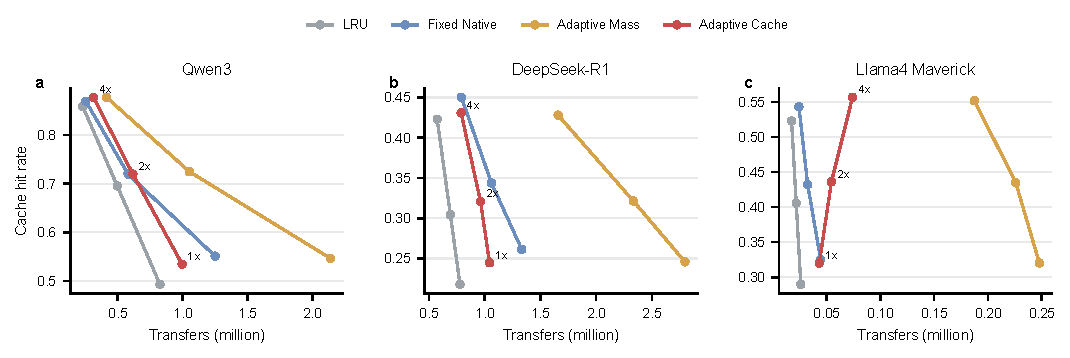
\includegraphics[width=0.94\textwidth]{figures/compact/Fig6_compact_cache_pareto}
\caption{Trace-driven cache Pareto analysis for (a) Qwen3, (b) DeepSeek-R1, and (c) Llama4 Maverick. Each curve contains cache capacities of $1\times$, $2\times$, and $4\times$; labels identify the adaptive-cache points. Upper-left movement is preferable because it combines higher hit rate with fewer transfers. Cache-aware rejection consistently reduces transfers relative to unfiltered adaptive mass, but the best policy depends on model and capacity.}
\label{fig:cache-pareto}
\end{figure*}

\FloatBarrier

\section{Discussion}
Discrete route histories retained predictive information across all three evaluated MoE families. TCN-only slightly improved over GRU-only in native-budget Recall, confirming that dilated temporal convolutions form a competitive history encoder. RouteCast nevertheless exceeded both models with paired confidence intervals above zero. The improvement therefore depends on more than the choice of recurrent or convolutional sequence encoder. Statistical priors stabilized sparse observations, temporal features captured recent deviations, and the gate adapted their contribution to context. No individual evidence branch was universally beneficial.

Forecasting quality and prefetch utility must nevertheless be evaluated separately. Wider candidate sets increased Recall but were particularly inefficient for DeepSeek-R1 and Top-1 Llama4 Maverick. Calibration made candidate scores comparable within each model. Rejection and cache-aware admission then determined whether a candidate justified speculative movement. Cache replay shows that this separation limits transfer amplification, but it does not guarantee universal system gains.

Three limitations bound these conclusions. First, public traces cannot measure transfer--compute overlap, exposed stalls, throughput, energy, or kernel overhead. Second, most scheduling and cache ablations use the limit=100 development setting; limit=1000 evidence currently covers the forecaster and primary baselines. Third, the learned comparators now include matched GRU and TCN models, but not a matched transformer. Limit=1000 multi-seed training and a current overhead benchmark remain necessary for a stronger systems claim.

\section{Conclusion}
RouteCast combines calibrated next-token expert forecasting with selective cache-aware prefetching. Under request-disjoint evaluation, it improved native-budget Recall, MRR, and NDCG across Qwen3, DeepSeek-R1, and Llama4 Maverick traces. Calibration and adaptive selection exposed the trade-off between coverage and speculative movement. Cache replay identified both transfer reductions and model-specific failure regions. These results support RouteCast as an algorithmic interface between forecasting and cache management, while end-to-end acceleration remains unverified.

\appendix
\section{Additional Evidence}
The accompanying supplementary figure package contains dataset composition, development-stage history sensitivity, limit=100 versus limit=1000 scale comparison, three-seed screening, legacy layer heterogeneity, calibration metrics, a legacy gate-overhead benchmark and the complete cache-replay tables. Legacy Qwen-only panels are labelled explicitly and are not used as evidence for the cross-model RouteCast V3 claim. The former 3-by-3 cache matrix is supplied separately rather than embedded as an unreadable composite figure.

\begin{figure}[!t]
\centering
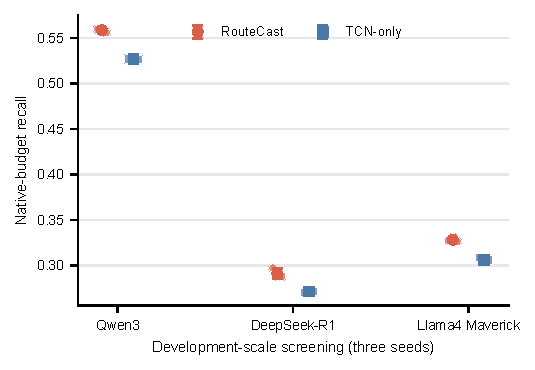
\includegraphics[width=0.95\columnwidth]{figures/split/FigS_tcn_seed_stability}
\caption{Development-scale stability screening over seeds 2024, 2025, and 2026. Small translucent points denote individual runs; large markers and error bars denote mean $\pm$ sample standard deviation. RouteCast exceeds the matched TCN-only baseline for all nine model--seed pairs.}
\label{fig:tcn-seeds}
\end{figure}

\begin{thebibliography}{00}
\bibitem{pregated} R. Hwang et al., ``Pre-gated MoE: An algorithm-system co-design for fast and scalable mixture-of-expert inference,'' in \emph{Proc. ISCA}, 2024.
\bibitem{moeinfinity} L. Xue et al., ``MoE-Infinity: Efficient MoE inference on personal machines with sparsity-aware expert cache,'' arXiv:2401.14361, 2024.
\bibitem{promoe} X. Song et al., ``ProMoE: Fast MoE-based LLM serving using proactive caching,'' arXiv:2410.22134, 2024.
\bibitem{patterns} Z. Yu et al., ``Patterns behind chaos: Forecasting data movement for efficient large-scale MoE LLM inference,'' arXiv:2510.05497, 2026.
\bibitem{specmd} D. Hoang et al., ``SpecMD: A comprehensive study on speculative expert prefetching,'' arXiv:2602.03921, 2026.
\bibitem{stmoe} Y. Zhao et al., ``A spatio-temporal expert prefetching framework for efficient MoE-based LLM inference,'' arXiv:2606.15453, 2026.
\bibitem{specprefetch} J. Kong et al., ``SpecPrefetch: Parameter-efficient expert prefetching for sparse MoE foundation models,'' arXiv:2607.24787, 2026.
\end{thebibliography}

\end{document}
